%% LyX 2.1.4 created this file.  For more info, see http://www.lyx.org/.
%% Do not edit unless you really know what you are doing.
\documentclass[english]{scrartcl}
\usepackage[T1]{fontenc}
\usepackage[latin9]{inputenc}
\usepackage{refstyle}
\usepackage{graphicx}

\makeatletter

%%%%%%%%%%%%%%%%%%%%%%%%%%%%%% LyX specific LaTeX commands.

\AtBeginDocument{\providecommand\secref[1]{\ref{sec:#1}}}
\AtBeginDocument{\providecommand\figref[1]{\ref{fig:#1}}}
\RS@ifundefined{subref}
  {\def\RSsubtxt{section~}\newref{sub}{name = \RSsubtxt}}
  {}
\RS@ifundefined{thmref}
  {\def\RSthmtxt{theorem~}\newref{thm}{name = \RSthmtxt}}
  {}
\RS@ifundefined{lemref}
  {\def\RSlemtxt{lemma~}\newref{lem}{name = \RSlemtxt}}
  {}


\@ifundefined{showcaptionsetup}{}{%
 \PassOptionsToPackage{caption=false}{subfig}}
\usepackage{subfig}
\makeatother

\usepackage{babel}
\begin{document}

\section{Model selection and Alignment\label{sec:Model-selection-and}}


\subsection{3D Model selection and pose estimation}

Crosslink/Manual/...


\subsection{Model Aligment and Scale}

Using 3D and 2D


\section{Refine aligment for Rendering}

After \secref{Model-selection-and}, we have a posed 3D model that
projected into the input cameras, it does approximate the ``actual''
shape present in the views but some silhouettes and internal edges
are misaligned (see \figref{Model-projection-into}).

\begin{figure}[h]
\begin{centering}
\subfloat[]{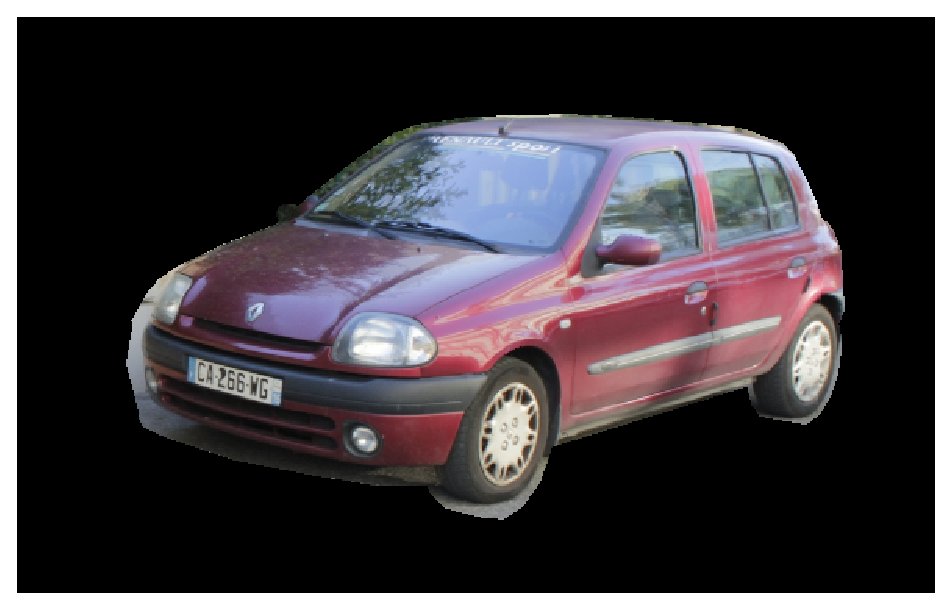
\includegraphics[width=5cm]{images/bopusquet_car_clio}



}
\par\end{centering}

\begin{centering}
\subfloat[]{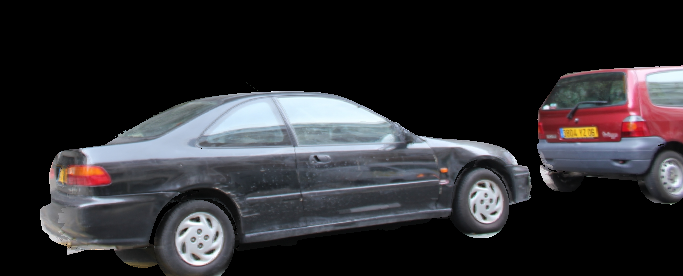
\includegraphics[width=5cm]{images/street10_honda-twingo}

}\subfloat[]{

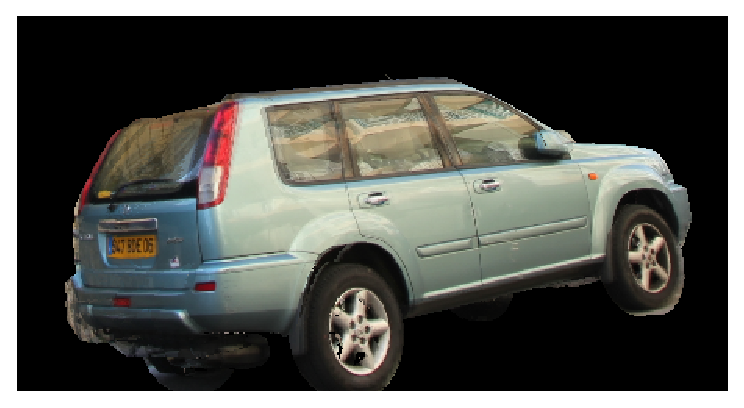
\includegraphics[width=5cm]{images/yellowshose12_nissan}

}\caption{Model projection into a input view after \secref{Model-selection-and}.\label{fig:Model-projection-into}}

\par\end{centering}

\centering{}
\end{figure}


Snakes 

Efros
\end{document}
